\documentclass[10pt]{article}

\usepackage[letterpaper,margin=0.86in]{geometry}
\usepackage{amsmath,amssymb,amsthm,mathtools}
\usepackage{booktabs,tabularx,array,multirow}
\usepackage{microtype}
\usepackage{enumitem}
\usepackage{listings}
\usepackage{xcolor}
\usepackage{hyperref}
\usepackage{url}
\usepackage{fancyhdr}
\usepackage{graphicx}
\usepackage{float}
\usepackage{tikz}
\usetikzlibrary{arrows.meta,positioning,fit}

\definecolor{accent}{HTML}{234A73}
\definecolor{soft}{HTML}{F4F6F8}
\definecolor{rulegray}{HTML}{D7DCE2}
\hypersetup{colorlinks=true,linkcolor=accent,citecolor=accent,urlcolor=accent,pdftitle={Operator-Level Boolean Computation with Correspondence Matrices},pdfauthor={Brian Theory}}
\setlength{\parindent}{1.05em}
\setlength{\parskip}{0pt}
\setlist{nosep,leftmargin=*}
\pagestyle{fancy}
\fancyhf{}
\fancyhead[L]{\small Operator-Level Boolean Computation with Correspondence Matrices}
\fancyhead[R]{\small Contract revision, 26 September 2026}
\fancyfoot[C]{\thepage}
\setlength{\headheight}{14pt}
\emergencystretch=2em

\newcommand{\B}{\mathbb B}
\newcommand{\Ftwo}{\mathbb F_2}
\newcommand{\bxor}{\mathbin{\Updownarrow}}
\newcommand{\ptop}[1]{\widehat{#1}}
\newcommand{\Pair}{\operatorname{Pair}}
\newcommand{\supp}{\operatorname{supp}}
\newcommand{\eval}{\mathcal E}
\newcommand{\IR}{\mathrm{IR}}
\newcommand{\AST}{\mathrm{AST}}
\newcommand{\true}{\mathrm{T}}
\newcommand{\false}{\mathrm{F}}

\theoremstyle{plain}
\newtheorem{theorem}{Theorem}
\newtheorem{lemma}{Lemma}
\newtheorem{proposition}{Proposition}
\theoremstyle{definition}
\newtheorem{definition}{Definition}
\theoremstyle{remark}
\newtheorem{remark}{Remark}

\lstset{
  basicstyle=\ttfamily\small,
  backgroundcolor=\color{soft},
  frame=single,
  rulecolor=\color{rulegray},
  columns=fullflexible,
  keepspaces=true,
  breaklines=true,
  xleftmargin=0.5em,
  xrightmargin=0.5em,
  aboveskip=0.7em,
  belowskip=0.7em
}

\title{\vspace{-1.3em}\textbf{Operator-Level Boolean Computation with Correspondence Matrices}\\[0.35em]
\large Typed operand frames, local operator folding, fallback semantics, and empirical boundaries}
\author{Brian Theory}
\date{Compiler contract and evidence revision --- 26 September 2026}

\begin{document}
\maketitle

\begin{abstract}
Correspondence matrices encode a binary Boolean connective as four bits in a declared operand frame. We specify a restricted compiler that normalizes signed and swapped variable occurrences, fuses tokens with matching frames, and distinguishes structural, tabulated, and hybrid derivations. An ordered strategy selects among those admissible derivations; failure of the selected strategy need not mean that no derivation exists. Soundness and completeness for an explicitly generated structural fragment are established using classical truth-function identities. The implementation contract separates syntactic variable occurrence from essential dependence, root pair success from discarded child constructions, and compact tokens from dense outputs over retained ambient axes. A pinned source snapshot and executable regression suite make these boundaries checkable. Recovered S1/S2 records show local reductions but a generic-optimizer tie; a separate ANF-dispatch study is negative overall. A prospectively frozen synthetic pair-token comparison on 64 held-out signed formulas also fails its primary utility rule: median direct-packed/CM production time is 0.248 (95\% hierarchical bootstrap interval 0.246--0.249). A separate correctness screen of 71 admitted original EPFL primary-output cones found four pure structural roots, one fully retabulated root, and 66 fallbacks. In a subsequently frozen descriptive secondary timing run, 70 cones completed paired full-bitset Python timing and one failed calibration; the complete-case median direct-packed/CM producer ratio was 0.0376, with direct evaluation faster on every complete case. ABC/AIG truth checking completed for all 71, but its subprocess wall time is not a matched producer comparison. The broader protocol-v3 systems comparison remains open. The contribution is a bounded compiler specification and reproducible negative systems boundary, not a new truth-table algebra or a demonstrated performance advantage.

\end{abstract}

\noindent\textbf{Draft status.} This is the revised compiler-focused manuscript after the deliberate CM/LM publication split. The companion foundations paper \emph{Correspondence and Logical Matrices: A Boolean Operator Calculus} owns the formula-valued LM theory, valuation, logical pairing, higher-arity tensors/maps, and the broader coherence calculus \cite{TheoryFoundations2026}. The present paper imports only the numeric binary contract required by the compiler. A narrower synthetic protocol-v4 confirmation is complete and negative. A natural-circuit admission/correctness gate and a separate, incomplete descriptive secondary timing run have since completed; the full timed protocol-v3 comparison has not.

\section{Introduction and claim boundary}

A binary Boolean connective contains four output values. A correspondence matrix stores those four values as a $2\times2$ array whose row and column axes are tied to declared operands. In isolation, that is only a reshaping of a truth table. The computational question is different: can a compiler use the small operator as a first-class token, normalize the token's operand frame, and combine compatible local operators before evaluating or expanding their operands?

The key example is deliberately simple. Consider
\begin{equation}
 (X\Rightarrow Y)\bxor(Y\Rightarrow X).
 \label{eq:mismatch-expression}
\end{equation}
Both inner connectives are implication, but they do not initially refer to the same ordered operand frame. Treating their four-bit arrays as if corresponding entries described the same assignment would be a type error. Once the second occurrence is transported from frame $(Y,X)$ to frame $(X,Y)$ by transpose, entrywise XOR is sound:
\begin{equation}
 [\Rightarrow]\,\ptop{\bxor}\,[\Rightarrow]^T=[\bxor].
 \label{eq:mismatch-fold}
\end{equation}
The resulting token represents $X\bxor Y$. Equation~\eqref{eq:mismatch-fold} is not important because XOR of two truth tables is difficult; it is important because it makes the \emph{admission condition} explicit. A local table may be fused only when its coordinates have a common logical meaning.

This paper therefore treats operand-frame metadata as part of the compiler type. A successful pair compilation returns not just four bits, but a token tied to canonical row and column operands. Swaps and input polarities are normalized by fixed reindexings. Compatible tokens can then be fused by an outer Boolean connective before repeated operand work or polynomial expansion. If structural recognition fails, the implementation can exactly retabulate an admitted two-variable subtree, can combine such a retabulated descendant with structural parents while marking the result hybrid, or can pass the original expression to the ordinary builder. Successful child pair constructions are not retained when the root pair attempt fails.

The component operations have substantial prior art. Boolean matrices predate this work \cite{Edwards1972}; matrix and vector logics represent logical operators algebraically \cite{Stern1988,Mizraji1992,Mizraji2008}; Cheng, Zhao, and Xu explicitly combine truth vectors entrywise under an arbitrary outer Boolean operation \cite{Cheng2011}; small truth functions, NPN transformations, LUTs, and DAG-aware rewriting are standard synthesis techniques \cite{Mishchenko2006,Zhou2019,Testa2019}; and bit-parallel evaluators compute several assignments simultaneously \cite{Lee2022}. Bricken's internally dated 1997 technical note is also a close antecedent for $2\times2$ logical matrices and bra--matrix--ket evaluation \cite{Bricken1997}. The present paper does not claim those ingredients as new.

The narrower contribution is computational and testable:
\begin{enumerate}
  \item a \textbf{typed frame-aware compiler rule} in which a four-bit CM token is paired with operand metadata and normalized before same-frame fusion;
  \item \textbf{sound multi-path semantics} separating pure structural compilation, local retabulation, hybrid composition, and ordinary fallback;
  \item an \textbf{executable implementation contract} separating compact tokens, framed surrogates, general IR, lowered programs, and ambient dense outputs, with regression tests for strategy selection, fixed axes, and discarded child constructions;
  \item \textbf{matched mechanism and negative evidence}: exploratory folding can reduce pre-expansion work, an equally capable generic optimizer can reproduce the same reductions, and frozen ANF-dispatch and synthetic pair-token studies show that local wins need not amortize; and
  \item a \textbf{preserved broader evaluation design} with natural admission, correctness, and bounded secondary producer timing now checked, while synthesis comparability, reuse, alternative outputs, memory, and fallback costs still require matched measurement.
\end{enumerate}

The scientific claim does not depend on CM folding being uniquely capable of a reduction. If a generic local truth-function optimizer reaches the same reduced form, that locates the mechanism in a broader family of small-function rewrites. The remaining CM-specific question is whether the representation and its frame metadata make recognition, legality, transformation, caching, or reuse sufficiently direct and inexpensive to matter in a full compiler.

\section{Minimal CM compiler contract}
\label{sec:minimal-contract}

The companion foundations paper develops the CM/LM calculus in detail \cite{TheoryFoundations2026}. Only the following binary numeric contract is required here.

Let
\begin{equation}
 \B=\{0,1\}\cong\Ftwo,
\end{equation}
with multiplication interpreted as conjunction and addition written as XOR, $\bxor$. For a bit $x\in\B$, use the true-first state
\begin{equation}
 |x\rangle=\begin{bmatrix}x\\ \neg x\end{bmatrix},
 \qquad
 \langle x|=\begin{bmatrix}x&\neg x\end{bmatrix}.
 \label{eq:state}
\end{equation}
For a binary logical connective variable $\Theta$, define the compact correspondence matrix
\begin{equation}
 [\Theta]
 :=
 \begin{bmatrix}
  \Theta_{11}&\Theta_{10}\\
  \Theta_{01}&\Theta_{00}
 \end{bmatrix}
 =
 \begin{bmatrix}
  1\Theta1&1\Theta0\\
  0\Theta1&0\Theta0
 \end{bmatrix}.
 \label{eq:cm}
\end{equation}
The row and column assignment order $(1,0)$ is part of the representation contract.

For $C\in\B^{2\times2}$, define the XOR--AND contraction
\begin{equation}
 \eval_C(x,y)=\langle x|C|y\rangle
 =\mathop{\bxor}_{r,s\in\{1,0\}}
 \chi_x(r)\wedge C_{rs}\wedge\chi_y(s),
 \label{eq:contraction}
\end{equation}
where $\chi_x(r)=1$ exactly when $r=x$.

\begin{proposition}[Selection]
For every binary connective $\Theta$ and $x,y\in\B$,
\begin{equation}
 \langle x|[\Theta]|y\rangle=x\Theta y.
 \label{eq:selection}
\end{equation}
\end{proposition}

\begin{proof}
Both states are one-hot. Every term in Equation~\eqref{eq:contraction} vanishes except the term at $(r,s)=(x,y)$.
\end{proof}

The compiler packs the four coefficients into a constant-size token. That token is not by itself sufficient to authorize a rewrite. An occurrence is also typed by an \emph{operand frame}: the row expression, column expression, their signed polarities, and the truth-state order. In the implementation considered here, a successful pair surrogate ultimately records canonical row and column variable names together with the normalized token.

\section{Typed normalization and same-frame fusion}
\label{sec:alignment}

Let
\begin{equation}
 P=\begin{bmatrix}0&1\\1&0\end{bmatrix}=[\bxor].
\end{equation}
Define $\Theta^\tau(x,y):=y\Theta x$. With the true-first convention,
\begin{align}
 [\Theta^\tau]&=[\Theta]^T, \\
 [\Theta(\neg X,Y)]&=P[\Theta], \\
 [\Theta(X,\neg Y)]&=[\Theta]P,
 \label{eq:input-transforms}
\end{align}
where products with $P$ are XOR--AND products and therefore act as row/column permutations. Output negation is entrywise complement.

For a binary outer connective $\Phi$, define same-position fusion by
\begin{equation}
 \bigl([\Theta_1]\ptop{\Phi}[\Theta_2]\bigr)_{rs}
 :=(\Theta_1)_{rs}\Phi(\Theta_2)_{rs}.
 \label{eq:pointwise}
\end{equation}
This is not matrix multiplication.

\begin{theorem}[Same-frame fusion]
If $[\Theta_1]$ and $[\Theta_2]$ are expressed in the same ordered operand frame, then for all $x,y\in\B$,
\begin{equation}
 (x\Theta_1 y)\Phi(x\Theta_2 y)
 =\left\langle x\middle|
 \left([\Theta_1]\ptop{\Phi}[\Theta_2]\right)
 \middle|y\right\rangle.
 \label{eq:fusion-theorem}
\end{equation}
\end{theorem}

\begin{proof}
Both sides select position $(x,y)$; the right-hand side stores the outer operation on exactly those two selected coefficients. No distributive law for $\Phi$ over XOR is required.
\end{proof}

The pointwise identity itself is classical; Cheng, Zhao, and Xu give the direct truth-vector antecedent in Proposition~3.3 \cite{Cheng2011}. The compiler-specific rule is therefore:

\begin{quote}
\textbf{Admission rule.} Transport signed/swapped occurrences to one declared frame. Apply Equation~\eqref{eq:fusion-theorem} only after row operand, column operand, polarity interpretation, and truth-state order agree.
\end{quote}

Figure~\ref{fig:compiler-flow} summarizes the resulting local pipeline.

\begin{figure}[H]
\centering
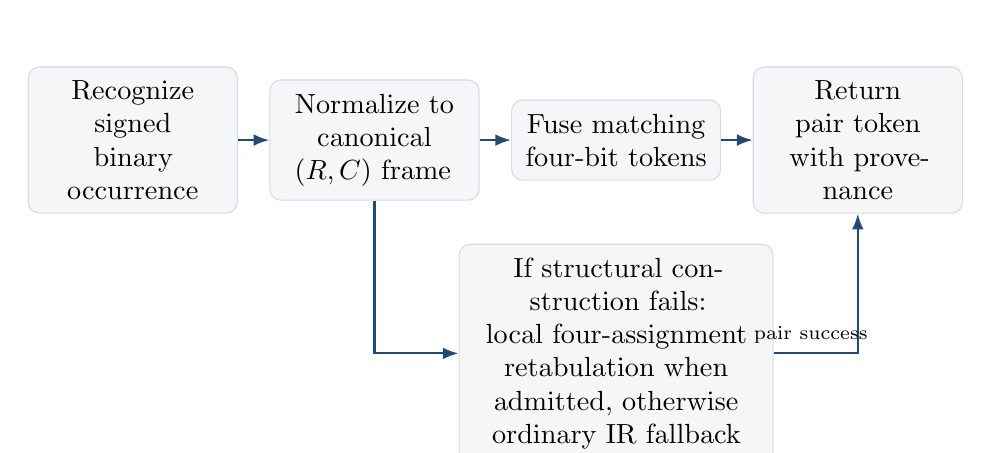
\begin{tikzpicture}[
 node distance=4mm and 4mm,
 box/.style={draw=rulegray,rounded corners,fill=soft,align=center,minimum height=10mm,text width=0.19\linewidth,inner sep=5pt},
 arrow/.style={-{Latex[length=2mm]},thick,draw=accent}
]
\node[box] (recognize) {Recognize signed\\binary occurrence};
\node[box,right=of recognize] (align) {Normalize to\\canonical $(R,C)$ frame};
\node[box,right=of align] (fuse) {Fuse matching\\four-bit tokens};
\node[box,right=of fuse] (out) {Return pair token\\with provenance};
\draw[arrow] (recognize)--(align);
\draw[arrow] (align)--(fuse);
\draw[arrow] (fuse)--(out);
\node[box,below=8mm of fuse,text width=0.30\linewidth] (fallback) {If structural construction fails:\\local four-assignment retabulation when admitted, otherwise ordinary IR fallback};
\draw[arrow] (align.south) |- (fallback.west);
\draw[arrow] (fallback.east) -| node[pos=0.22,above,font=\scriptsize]{pair success} (out.south);
\end{tikzpicture}
\caption{The compiler transformation. The operation performed on the four-bit token is trivial; the semantic work is the typed recognition and normalization that determines when fusion is legal and what fallback is required.}
\label{fig:compiler-flow}
\end{figure}

\subsection{Why frame metadata matters}

Return to Equation~\eqref{eq:mismatch-expression}. The two implication tokens are numerically equal before typing, but the second occurrence's array coordinates refer to $(Y,X)$ rather than $(X,Y)$. Naively XORing the two unaligned arrays would return the zero token. Transposition moves the second operator into the target frame, after which Equation~\eqref{eq:mismatch-fold} correctly yields $[\bxor]$. The error is therefore not a deficiency of truth tables; it is a failure to track which assignment each stored bit denotes.

This distinction is closely related to established NPN-style input permutation/negation and output-negation operations \cite{Mishchenko2006,Zhou2019}. The present use is intentionally narrower than a general NPN canonicalizer. It treats frame transport as a local typing obligation for a particular rewrite.

\section{Pair compiler and soundness}
\label{sec:compiler}

\subsection{Judgment, invariant, and provenance}

Let expressions use the grammar
\begin{equation}
 e ::= Z\mid \neg e\mid e\,\Phi\,e,
 \label{eq:grammar}
\end{equation}
where $Z$ is a variable and $\Phi$ is one of the currently supported binary connectives AND, OR, XOR, implication, and equivalence. Fix distinct canonical variables $R$ and $C$ and a fixed-substitution map $F$ that binds neither variable on a returned pair path. Write $\Gamma=(R,C,F)$.

Let $\operatorname{Vars}(e)$ collect variable names occurring in the source syntax, recursively by singleton, identity through negation, and union through a binary node. Define
\begin{equation}
 \supp_F(e):=\operatorname{Vars}(e)\setminus\operatorname{dom}(F).
 \label{eq:syntactic-support}
\end{equation}
This is \emph{syntactic unfixed occurrence}, not essential functional dependence. No Boolean simplification is implicit: $X\lor(Y\bxor Y)$ still has support $\{X,Y\}$ when $F$ is empty, although its value depends only on $X$. Fixed names are excluded from this set and their values are supplied during evaluation.

An admissible typed pair derivation has judgment
\begin{equation}
 \Gamma\vdash e\Downarrow^p \Pair(R,C,t),
 \qquad p\in\{S,T,H\},
 \label{eq:judgment}
\end{equation}
with the intended invariant
\begin{equation}
 \eval_t(r,c)=e[r/R,c/C]
 \quad\text{for all }r,c\in\B,
 \label{eq:invariant}
\end{equation}
interpreted after the fixed substitutions in $F$.

Equation~\eqref{eq:judgment} can be read as follows: under compiler environment $\Gamma$, expression $e$ admits a derivation of the four-bit token $t$ in canonical frame $(R,C)$, and $p$ records how that token was obtained. Equation~\eqref{eq:invariant} is the semantic contract. Each of the four token positions must return exactly the value of the original expression under the corresponding assignment to $R$ and $C$. The pair therefore carries both a compact Boolean function and the frame metadata needed to interpret its bit positions.

The provenance values are:
\begin{itemize}
 \item \textbf{$S$ --- structural:} the returned subtree used signed primitive recognition, token complement, and/or same-frame fusion only.
 \item \textbf{$T$ --- tabulated root:} the returned subtree itself was produced by evaluating all four assignments. The symbol $T$ avoids overloading $R$, which already denotes the row variable.
 \item \textbf{$H$ --- hybrid:} structural steps occur above at least one tabulated descendant.
\end{itemize}
The judgment is a relation, not a deterministic strategy. For example, $X\land Y$ admits both an $S$ primitive derivation and a $T$ tabulation derivation, with the same token $1000_2$. Section~\ref{sec:selection} specifies which derivation is selected. The token API returns \texttt{None} with diagnostic \texttt{ordinary\_fallback} if the selected procedure returns no pair; it does not itself execute the ordinary builder.

\subsection{Rules, built up one step at a time}

The inference-rule bar is read as implication: if the premises above the bar hold, the compiler may derive the conclusion below it. The rules perform four conceptually distinct jobs: create a normalized primitive token, complement an already compiled token, fuse two already aligned tokens, and tabulate an exact two-variable subtree. Their validity is independent of the order in which an implementation attempts them.

\paragraph{Primitive normalization.}
Let $\ell_1,\ell_2$ be signed literals whose underlying variables are exactly $R$ and $C$ in either order. If the declared normalization procedure transports the primitive occurrence $\Theta(\ell_1,\ell_2)$ into the canonical frame and returns token $t$, then the compiler may derive
\[
\frac{
  \operatorname{Norm}_{\Gamma}(\Theta(\ell_1,\ell_2))=t
}{
  \Gamma\vdash \Theta(\ell_1,\ell_2)\Downarrow^S \Pair(R,C,t)
}.
\]
Normalization consists only of the declared operand exchange and row/column polarity transforms from Equation~\eqref{eq:input-transforms}. This is the structural base case: it establishes a token whose four bit positions already refer to the canonical assignments $(R,C)=(1,1),(1,0),(0,1),(0,0)$.

\paragraph{Negation: Equation~\eqref{eq:neg-rule}.}
Once a child has a correct token in the canonical frame, negating the expression requires only bitwise complement of that token:
\begin{equation}
\frac{\Gamma\vdash a\Downarrow^p\Pair(R,C,t_a)}
{\Gamma\vdash \neg a\Downarrow^{\nu(p)}\Pair(R,C,\neg t_a)}.
\label{eq:neg-rule}
\end{equation}
The frame does not change. Here $\neg t_a$ means complement each of the four token bits. Provenance changes only to report ancestry: $\nu(S)=S$ and $\nu(T)=\nu(H)=H$. Thus a structural NOT above a locally tabulated child is correct but explicitly reported as hybrid.

\paragraph{Same-frame fusion: Equation~\eqref{eq:fuse-rule}.}
Two compiled children may be fused only when their pair metadata name the same canonical frame:
\begin{equation}
\frac{\Gamma\vdash a\Downarrow^p\Pair(R,C,t_a)
\qquad
\Gamma\vdash b\Downarrow^q\Pair(R,C,t_b)}
{\Gamma\vdash a\Phi b\Downarrow^{p\sqcup q}\Pair(R,C,t_a\ptop{\Phi}t_b)}.
\label{eq:fuse-rule}
\end{equation}
The token operation $t_a\ptop{\Phi}t_b$ applies $\Phi$ independently to corresponding token positions. The repeated $\Pair(R,C,\cdot)$ in the two premises is the essential admission certificate: position $11$ in one child denotes the same assignment as position $11$ in the other, and similarly for $10,01,00$. Define $S\sqcup S=S$; every other combination is $H$ because tabulated ancestry is present below a structural fusion.

\paragraph{Exact local tabulation.}
If the syntactic unfixed support $\supp_F(e)$ is exactly $\{R,C\}$, define the true-first token
\begin{equation}
 t_e:=\bigl(e(1,1),e(1,0),e(0,1),e(0,0)\bigr).
 \label{eq:tab-token}
\end{equation}
Then the exact tabulation rule is
\[
\frac{
  \supp_F(e)=\{R,C\}
  \qquad t=t_e
}{
  \Gamma\vdash e\Downarrow^T\Pair(R,C,t)
}.
\]
This rule re-evaluates a two-variable subtree on its complete four-assignment domain. It is an exact semantic base case. Its rule has no premise requiring structural failure; that restriction belongs to the ordered hybrid procedure.

\paragraph{Worked derivation.}
Let $\Gamma=(X,Y,\varnothing)$ and
\begin{equation}
 e=(X\Rightarrow\neg Y)\bxor(\neg Y\Rightarrow X).
 \label{eq:worked-expression}
\end{equation}
In true-first order $(11,10,01,00)$, implication has token $1011_2$. For the left child, the variables are already in $(X,Y)$ order but the column literal is negated, so the column-polarity transform gives
\[
 X\Rightarrow\neg Y\quad\longmapsto\quad 0111_2.
\]
For the right child, the source operands arrive as $(\neg Y,X)$. Operand exchange followed by polarity alignment gives
\[
 \neg Y\Rightarrow X\quad\longmapsto\quad 1110_2.
\]
Both children now carry frame $(X,Y)$, so Equation~\eqref{eq:fuse-rule} is legal:
\begin{equation}
 0111_2\ \bxor\ 1110_2=1001_2.
 \label{eq:worked-fusion}
\end{equation}
Hence
\[
 \Gamma\vdash e\Downarrow^S\Pair(X,Y,1001_2).
\]
The token $1001_2$ is $[\Leftrightarrow]$ in true-first order, so the compiler has established
\[
 (X\Rightarrow\neg Y)\bxor(\neg Y\Rightarrow X)=X\Leftrightarrow Y
\]
without first expanding the source expression into an ANF or another larger symbolic representation. Applying Equation~\eqref{eq:neg-rule} once more complements $1001_2$ to $0110_2$, the XOR token.

An $S$ derivation uses no tabulation; a $T$ derivation ends with tabulation; an $H$ derivation uses structural composition above a tabulated descendant. These are derivation properties. In particular, the strategy named \texttt{hybrid} can select an $S$, $T$, or $H$ result, depending on the expression.

\begin{theorem}[Pure structural soundness]
If $\Gamma\vdash e\Downarrow^S\Pair(R,C,t)$, then Equation~\eqref{eq:invariant} holds and no four-assignment tabulation was used.
\end{theorem}

\begin{proof}
Induct on the derivation. A signed primitive is correct by the frame transforms in Equation~\eqref{eq:input-transforms}; complementing a correct child represents negation; and fusing two correct children with identical metadata is sound by Theorem~1.
\end{proof}

\begin{definition}[Declared pure-structural fragment]
Fix canonical variables $R,C$. Let $\mathcal S_{R,C}$ be the smallest expression class containing every supported primitive $\Theta(\ell_1,\ell_2)$ whose signed literals have underlying variables exactly $R,C$ in either order, and closed under negation and the five supported binary connectives.
\end{definition}

\begin{theorem}[Completeness for the declared pure-structural fragment]
For every $e\in\mathcal S_{R,C}$, the \texttt{pure\_structural} strategy derives a unique canonical-frame token $t$ such that
\[
 \Gamma\vdash e\Downarrow^S\Pair(R,C,t)
\]
and Equation~\eqref{eq:invariant} holds.
\end{theorem}

\begin{proof}
Induct on the construction of $e$. Every primitive in $\mathcal S_{R,C}$ is admitted by primitive normalization. Negation preserves the frame and remains structural by Equation~\eqref{eq:neg-rule}. If two children belong to $\mathcal S_{R,C}$, induction gives tokens in the same canonical frame, so Equation~\eqref{eq:fuse-rule} applies. Uniqueness follows because a Boolean function on fixed variables $R,C$ has one four-bit truth token in the declared true-first order.
\end{proof}

\begin{remark}
This is syntactic completeness for the deliberately declared compiler fragment, not semantic completeness for all formulas with two-variable support. A semantically equivalent expression outside $\mathcal S_{R,C}$ may still require exact tabulation or ordinary fallback.
\end{remark}

\begin{lemma}[Exact pair tabulation]
Suppose the syntactic unfixed support $\supp_F(e)$ is exactly one distinct row variable $R$ and one distinct column variable $C$. Evaluating $e$ at $(1,1),(1,0),(0,1),(0,0)$ and storing those four outputs in true-first order produces the unique token satisfying Equation~\eqref{eq:invariant}.
\end{lemma}

\begin{theorem}[Soundness of admitted pair compilation]
Every derivable pair result with provenance $p\in\{S,T,H\}$ satisfies Equation~\eqref{eq:invariant}. Separately, if the selected procedure returns no pair, the dense wrapper delegates correctness to the unchanged ordinary IR evaluator on the original expression, assuming that evaluator's contract.
\end{theorem}

\begin{proof}
The cases $S$ and $T$ are the preceding theorem and lemma. For $H$, use structural induction with exact local tabulation as an additional sound base case; token complement and same-frame fusion preserve the invariant. Provenance changes the reported construction path, not the represented function. The fallback statement is an interface contract rather than a theorem about the pair compiler itself.
\end{proof}

\subsection{Admissibility boundary}

The current pure structural rule does not claim semantic recognition of arbitrary equivalent compound operands. Repeated-variable forms such as $X\Theta X$, opaque compound operands, and incompatible variable pairs remain outside the pure rule. Duplicate axes and overlapping row/column layouts are invalid inputs and raise an error; they are not ordinary pair misses. A retabulation rule may cover some two-variable cases exactly, but it is intentionally classified as a different mechanism.

This conservative boundary is useful. It allows the compiler to refuse a local rewrite rather than infer an unproved equivalence. It also gives the experiment a measurable fallback frequency instead of hiding unsupported cases in preprocessing.

\section{Implementation architecture and cost model}
\label{sec:implementation}

\subsection{Five artifacts, not one}

Table~\ref{tab:artifacts} separates implementation objects that are easily conflated when all are described informally as a ``CM.''

\begin{table}[t]
\centering
\small
\begin{tabularx}{\linewidth}{@{}>{\raggedright\arraybackslash}p{0.18\linewidth}>{\raggedright\arraybackslash}X >{\raggedright\arraybackslash}p{0.24\linewidth}@{}}
\toprule
\textbf{Artifact} & \textbf{Meaning} & \textbf{Role}\\
\midrule
CM operator token & One binary truth function packed into four true-first bits $(11,10,01,00)$. & Constant-size transform and fusion.\\
Pair surrogate & Token plus canonical row and column operand names/frame metadata. & Carries the legality invariant.\\
General CM/Boolean IR & Interned expression DAG for arbitrary supported formulas. & General symbolic fallback and compilation.\\
Flat program & Backend-dependent instruction sequence lowered from the IR. & Repeated packed/array evaluation.\\
Explicit dense output & Materialized truth relation over all retained ambient row/column axes. & $2^m$ entries for $m$ retained axes; one byte per NumPy Boolean entry.\\
\bottomrule
\end{tabularx}
\caption{Compiler artifacts and their semantic boundaries. Only the first is the constant-size binary operator token.}
\label{tab:artifacts}
\end{table}

A token-only endpoint cannot be compared as if it had already paid to construct an explicit $2^m$-entry ambient result. Conversely, a comparator that has already prepared a reusable DAG or program should not be charged for that preparation on every query when the CM arm is allowed resident reuse. Endpoint equality is part of benchmark correctness.

\subsection{Ordered, strategy-dependent selection}
\label{sec:selection}

The source snapshot is pinned to commit \texttt{0ab8ffd0c23ffa71ee951d375b1c170ffdcc084b} of the public implementation \cite{CompilerSnapshot2026}. Let $\mathcal R,\mathcal C$ be ordered ambient row/column name lists, each duplicate-free and mutually disjoint. A pair frame consists of one unfixed name $R\in\mathcal R$ and one unfixed name $C\in\mathcal C$; these names are discovered from the expression, not chosen by lexicographic order. The full supported AST is validated and its occurrence, identity-node, and height statistics are computed before strategy selection. The intended input domain supplies every occurring name through a layout or $F$; other errors are not silently converted into pair misses.

\begin{lstlisting}
Pair(e, row_layout, column_layout, F, allowRetab):
    if e is a supported binary connective over signed literals
       with distinct unfixed names on opposite layout sides:
        normalize operand order and polarities
        return Pair(R, C, token, S)
    if e = NOT a:
        child = Pair(a, ..., allowRetab)
        if child succeeds: return its complement, with nu provenance
    else if e = a Phi b:
        left  = Pair(a, ..., allowRetab)
        right = Pair(b, ..., allowRetab)  # attempted even if left fails
        if both succeed on the same frame:
            return their fusion, with joined provenance
    else if e is a variable: return NoPair
    else: raise unsupported-node error
    if allowRetab and supp_F(e) has exactly one row and one column name:
        return four-assignment token with provenance T
    return NoPair

Select(e, strategy):
    pure_structural -> Pair(e, ..., allowRetab=false)
    hybrid          -> Pair(e, ..., allowRetab=true)
    retabulate      -> tabulate root if support admits a pair, else NoPair
\end{lstlisting}

The compatibility name \texttt{structural} aliases \texttt{hybrid}, not \texttt{pure\_structural}. For valid input and fixed strategy, the procedure selects one outcome. Every successful return supplies a derivation of Equation~\eqref{eq:judgment}: this follows by induction over the executed recursive calls, using the corresponding inference rule at each return. Thus the relational soundness theorems apply to the selected result. A \texttt{NoPair} return means failure of that strategy, not non-derivability in the entire relation. For example, $X\lor(Y\land Y)$ has a $T$ derivation but the pure strategy returns \texttt{NoPair}. Recursion terminates on finite acyclic ASTs/DAGs; the recursive pair walk can revisit identity-shared nodes.

\paragraph{Selection, diagnostics, and commitment.}
The public token artifact stores the two names and token; provenance is returned in accompanying metrics. Selected $S,T,H$ map respectively to \texttt{pure\_structural}, \texttt{full\_retabulation}, and \texttt{hybrid\_pair}. \texttt{None} maps to \texttt{ordinary\_fallback}, even in the token-only API, where no builder is called. The dense wrapper first checks the ambient output budget, then obtains the token result. On success it lifts that token to the ambient layout; on failure it calls the ordinary builder on the \emph{original expression}.

Consequently, $e=(X\land Y)\lor Z$, with no fixed variables and layouts $[X,Z]$ and $[Y]$, constructs an $S$ child for $X\land Y$ but returns no root pair. The successful child is discarded when the dense wrapper invokes the builder. The builder may independently optimize the original expression; this wrapper does not pass it a partially rewritten tree. Likewise, a root retabulation can supersede earlier child attempts. Counters such as \texttt{pair\_collapses} measure local work performed, including discarded work, not committed rewrites in the returned object. Root outcome must accompany these counters; committed contributions require separate instrumentation. Persistent child rewriting would be a different compiler version.

\subsection{Layout conversion and ownership}

The compact token uses true-first order while the historical dense array path uses false-first axes. The conversion is an explicit reindexing. If $T$ denotes the true-first $2\times2$ view and $D$ the false-first view indexed by array positions $a,b\in\{0,1\}$, then
\begin{equation}
 D_{ab}=T_{1-a,1-b}.
 \label{eq:layout-conversion}
\end{equation}
The dense contract retains \emph{every supplied ambient axis}, including fixed names and names on which the residual function is independent. Writing $m=|\mathcal R|+|\mathcal C|$, the returned shape is
\begin{equation}
 2^{|\mathcal R|}\times2^{|\mathcal C|},\qquad\text{with }2^m\text{ Boolean entries}.
 \label{eq:ambient-shape}
\end{equation}
For each false-first row/column index, decode its ambient assignment, override fixed names by $F$, and evaluate $e$. This defines the corresponding entry. Fixed values affect evaluation, while their axis positions remain and repeat that value; irrelevant axes are also broadcast. A fixed variable may be supplied by $F$ without appearing in the layout.

For example, $(X\land Y)\lor Z$ with $F=\{Z\mapsto0\}$, $\mathcal R=[X,Z]$, and $\mathcal C=[Y]$ returns
\begin{equation}
 M=\begin{bmatrix}0&0\\0&0\\0&1\\0&1\end{bmatrix},
 \label{eq:fixed-axis-example}
\end{equation}
whose rows are $(X,Z)=00,01,10,11$. The residual function is $X\land Y$, but the result has eight entries. A projected four-entry relation would require the caller to request a reduced layout or a separately specified projection API. The current dense wrapper neither drops fixed axes nor minimizes essential support.

The materialized dense result is an owned writable array, not a writable broadcast view. Its NumPy Boolean entries occupy one byte each; a bit-packed relation is a different output representation. Expression nodes and pair surrogates are immutable under the compiler contract, and caller-owned layouts/fixed maps are read-only.

\subsection{Cost model}

Let $N$ be AST occurrences, $U$ unique DAG nodes, $H$ AST height, $S$ occurrences in a subtree sent to retabulation, $D$ its evaluation depth, $k$ the length of a signed literal's negation chain, and $m$ the number of retained ambient output axes. The counts $|\supp_F(e)|$ and the number of essential variables can both be smaller than $m$.

\begin{itemize}
 \item Inspecting a signed literal costs $O(k)$ followed by an $O(1)$ four-bit transform.
 \item A four-bit token fusion is $O(1)$.
 \item One exact pair retabulation costs $O(4S)$ time plus the evaluator's stack/workspace requirements.
 \item A fully successful structural pair tree is ordinarily $O(N)$ time and $O(H)$ stack space, although the current support-discovery strategy can rescan rejected subtrees and therefore has an $O(N^2)$ worst case.
 \item A sharing-aware evaluator may scale with $U$ rather than $N$, which is why DAG-preserving packed/CSE comparators are mandatory.
 \item The current dense wrapper budgets and materializes $2^m$ entries even if many are repeated. Its output allocation/copy costs $\Theta(2^m)$ time and bytes; additional compiler workspace is separate. Projected or bit-packed outputs require separate accounting.
\end{itemize}

The last point prevents a common category error: constant-time token fusion is a local kernel fact, not an end-to-end complexity theorem.

\section{Closest prior art and matched comparators}
\label{sec:related}

The compiler should be compared with operations that possess equivalent local information, not with deliberately weaker baselines.

\paragraph{Boolean matrices and truth vectors.}
Edwards developed Boolean-matrix logic well before the present work \cite{Edwards1972}. Cheng, Zhao, and Xu use XOR as addition and AND as multiplication and state the same-variable entrywise outer-operation law in Proposition~3.3 \cite{Cheng2011}. Reshaping such a vector into $2\times2$ form does not make that pointwise identity new.

\paragraph{Matrix/vector logic.}
Stern and Mizraji provide established operator/matrix representations of logic \cite{Stern1988,Mizraji1992,Mizraji2008}. Bricken's technical note explicitly places logical matrices between two-component states in bra--matrix--ket form \cite{Bricken1997}. The companion foundations paper contains the appropriate broader comparison; the computational manuscript needs only enough of this history to prevent novelty from being attached to notation or representation alone.

\paragraph{NPN, LUT, and AIG practice.}
Small truth functions are routinely packed into machine words, transformed under input permutation/negation and output negation, classified up to NPN equivalence, and used in cut-based rewriting. DAG-aware AIG rewriting specifically exploits graph sharing rather than treating a formula as an unshared tree \cite{Mishchenko2006,Zhou2019,Testa2019}. CM transposition, row/column reversal, complement, and four-bit storage are therefore familiar small-function operations. Kitty directly provides truth-table Boolean operations, variable swaps/flips, dependence tests, cofactors, and base expansion \cite{KittyOperations}. These primitives do not distinguish this compiler.

The closest architectural comparison also carries operand identity: mockturtle cut rewriting supplies a truth table together with an ordered iterator range of leaves \cite{MockturtleCut}. An explicit frame is therefore not an unprecedented addition to a truth function. DAG-aware AIG rewriting evaluates candidate replacement gain against shared graph structure before committing a selected replacement \cite{Mishchenko2006}. The present wrapper instead attempts a restricted variable-pair root and abandons child constructions on root failure; it neither enumerates general cuts nor selects network replacements by sharing-aware area gain.

\begin{table}[H]
\small\centering
\begin{tabularx}{\linewidth}{@{}p{0.23\linewidth}XX@{}}
\toprule
\textbf{Comparison} & \textbf{Shared capability} & \textbf{Boundary in this paper}\\
\midrule
Cheng et al.; kitty & Aligned truth-function combination and table manipulation. & No algebraic or primitive-operation novelty claim.\\
Cut/AIG rewriting & Truth functions with leaf identities, input transforms, local candidates. & No general cut enumeration, gain search, or persistent graph replacement here.\\
Direct packed/DAG evaluator & Same four values; identity sharing can be preserved. & Primary end-to-end comparator; recognition overhead must be paid.\\
This contract artifact & Frame, strategy, provenance, failure, ownership, and output size specified together. & Regression-tested integration; synthetic primary and bounded natural secondary comparisons are negative.\\
\bottomrule
\end{tabularx}
\caption{Closest comparisons and the remaining, deliberately limited methods contribution. No kitty or AIG runtime comparison was executed for this revision.}
\end{table}

\paragraph{Direct packed evaluation.}
A strong simple comparator evaluates the AST once over four packed masks to obtain all four assignments in parallel. With identity memoization it also preserves explicit DAG sharing. It returns exactly the same four-bit function required by a pair-token endpoint and does not need CM-specific frame metadata. This is the closest baseline for deciding whether structural recognition pays for itself.

\paragraph{Generic local truth-function optimization.}
A generic optimizer given the same local support/function information can tabulate or combine a small cut without using CM notation. The S1/S2 evidence below shows why this comparator is scientifically necessary: it reaches the same reduced symbolic outputs as CM folding on the admitted all-arm cases.

\paragraph{ROBDDs and broader rewrite search.}
ROBDDs provide canonical function representations for a fixed variable order \cite{Bryant1986}. Equality saturation and synthesis-driven superoptimization retain or search broader classes of equivalent expressions \cite{Willsey2021,Sasnauskas2017}. These systems solve a more general problem than the fixed two-operand rule; comparison should therefore charge recognition/search/extraction and compare delivered artifacts appropriate to the task.

\section{Experimental questions and evidence hierarchy}
\label{sec:evaluation}

The computational claim is meaningful only if the benchmark answers the same question for every arm. Four distinctions are especially important.

\begin{enumerate}
 \item \textbf{Kernel versus compiler.} Four-bit fusion time is not compilation time.
 \item \textbf{Prepared versus one-shot.} A resident token/program may amortize setup; one-shot use may not.
 \item \textbf{Compact versus materialized output.} A token endpoint is not a complete $2^m$-entry ambient truth relation.
 \item \textbf{Task contract.} ANF production, complete truth-vector evaluation, repeated restriction, counting, and multi-root output are different tasks and cannot share one headline ratio.
\end{enumerate}

Figure~\ref{fig:evidence-levels} shows the evidence levels used in this draft.

\begin{figure}[H]
\centering
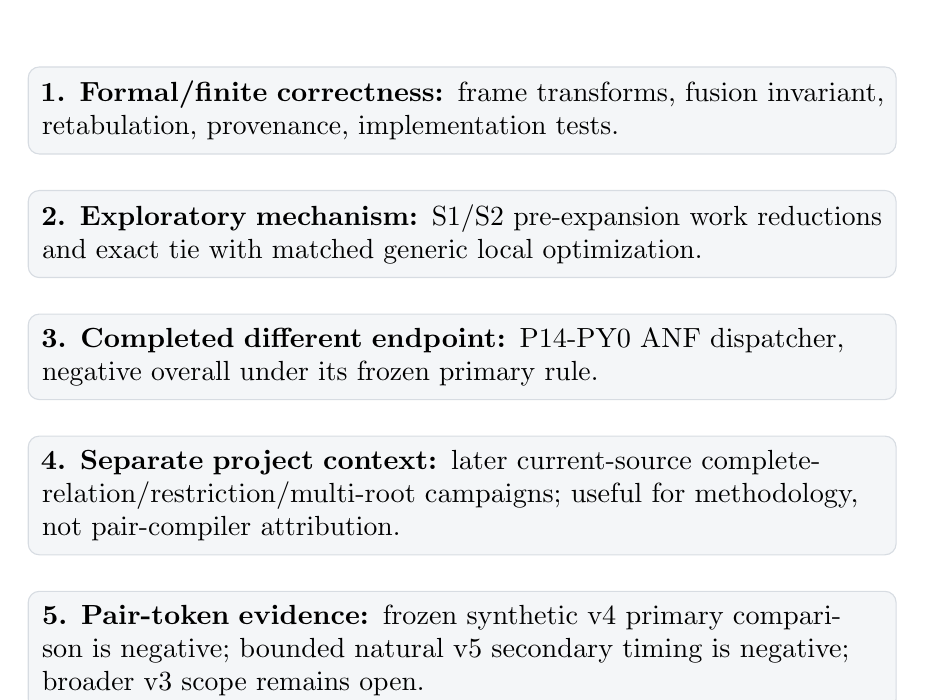
\begin{tikzpicture}[
 node distance=4.5mm,
 level/.style={draw=rulegray,rounded corners,fill=soft,align=left,text width=0.88\linewidth,inner sep=5pt},
]
\node[level] (a) {\textbf{1. Formal/finite correctness:} frame transforms, fusion invariant, retabulation, provenance, implementation tests.};
\node[level,below=of a] (b) {\textbf{2. Exploratory mechanism:} S1/S2 pre-expansion work reductions and exact tie with matched generic local optimization.};
\node[level,below=of b] (c) {\textbf{3. Completed different endpoint:} P14-PY0 ANF dispatcher, negative overall under its frozen primary rule.};
\node[level,below=of c] (d) {\textbf{4. Separate project context:} later current-source complete-relation/restriction/multi-root campaigns; useful for methodology, not pair-compiler attribution.};
\node[level,below=of d] (e) {\textbf{5. Pair-token evidence:} frozen synthetic v4 primary comparison is negative; bounded natural v5 secondary timing is negative; broader v3 scope remains open.};
\end{tikzpicture}
\caption{Evidence hierarchy. A favorable result on a different endpoint is not promoted into pair-compiler evidence.}
\label{fig:evidence-levels}
\end{figure}

\subsection{Confirmatory workload design}

The preserved, pre-freeze protocol-v3 design \cite{ProtocolV3} separates exact-frame formulas, signed/swapped frames, local retabulation cases, hybrid mixed-child cases, multiple operand pairs, compound-operand cases outside the structural claim, and natural formulas/circuits. Balanced generated trees use AST occurrence counts $15,63,255,1023,4095$; skewed trees stop at 255 occurrences and measured height at most 128. Cases cross the five supported outer connectives, reuse counts $1,10,100,1000$, and sharing conditions that distinguish identity-shared nodes, structurally equal but separately allocated subtrees, and no sharing. Every case records both $N$ and $U$.

Requested outputs include compact tokens, scalar evaluation, packed batches, and dense outputs where the output budget permits them. Preparation and query costs are reported separately. Once two arms have produced the same four-bit token and call the same lookup function, the query cost is common; any advantage must arise earlier or through a measured reuse policy.

The sole primary cell is intentionally narrow: signed/permuted pure-structural balanced formulas with $N=1023$, $U=N$, no fixed variables, token output, reuse one, compared end to end with direct packed AST evaluation. The proposed primary success rule requires zero correctness disagreements, a median competitor-to-CM ratio of at least $1.20$ whose 95\% interval lies entirely above one, and no more than a 10\% median peak-memory increase. The interval requirement establishes superiority, not a lower confidence guarantee of $1.20\times$. All other cells are secondary. This prevents a favorable post hoc workload from replacing a failed primary comparison.

A dated protocol-v4 successor fixed the synthetic primary case count and seeds, resident cache-reset timing, formula-level aggregation, and resampling before timing held-out formulas; Section~\ref{sec:v4-primary} reports its negative result. A separately frozen EPFL primary-output admission and correctness screen reports root outcomes by strategy (Section~\ref{sec:natural-gate}). A later frozen descriptive v5 run measures matched Python full-bitset production on 70 of the 71 selected cones, retaining one calibration failure; ABC process wall remains an unmatched diagnostic. Admission addresses applicability rather than timing superiority.

The $1.20\times$ ratio and 10\% memory allowance are engineering acceptance targets, not consequences of soundness or a power calculation. Their purpose is to demand a material gain while limiting memory growth; a $1.20\times$ ratio corresponds to 16.7\% less elapsed time. The preserved plan did not establish an empirical power calculation. The v4 pilot used disjoint seeds and met the 5\% repeatability criterion on its eight cases; the 64 formula/case seeds, rather than timing repetitions, supply the independent units for the reported synthetic interval. Its negative result is retained under the originally declared threshold.

\paragraph{Initialization and cache regimes.}
The source builds composition lookup tables when \path{cm_token} is imported, memoizes \path{cm_compose}, and caches permutation/lift metadata in \path{cm_normalize}. A fresh-process one-shot measurement must charge startup/import and table initialization. V4 instead uses a fresh process per formula but times repeated calls after common imports, clearing the CM memoization before each CM call and the bitset-environment cache before each direct call. The direct timed call builds its environment; imported lookup tables remain resident and their setup is recorded separately. This is a post-import cache-reset comparison, not a full process-start comparison. Warm regimes require a declared priming workload and cache lifetime. Charge support discovery, recognition, unsuccessful pair work, retabulation, fallback, and required materialization to their respective production arms; separate common token queries from preparation.

\section{Current evidence}
\label{sec:results}

\subsection{Correctness and implementation assurance}
\label{sec:fresh-checks}

The historical record reports 116 focused tests on 19 September 2026 and a separate 1,048,576-case signed-fusion check. Those reports do not by themselves bind that historical execution to the source revision inspected here. This revision supplies a fresh, separately identified run against the unmodified pinned source: 90 upstream tests from \texttt{test\_cm\_pair\_alignment.py} and \texttt{test\_output\_budget.py}, plus 33 contract regression cases, all passed. The latter include an exhaustive comparison over all 16 input tokens in each of eight signed frames, both children, all five supported outer connectives, and all four assignments: 327,680 scalar comparisons. This is implementation correctness evidence, not a timing campaign or a rerun of the historical 116-test selection.

\begin{table}[H]
\small\centering
\begin{tabularx}{\linewidth}{@{}p{0.34\linewidth}XXX@{}}
\toprule
\textbf{Expression / boundary} & \textbf{Pure} & \textbf{Hybrid} & \textbf{Retabulate}\\
\midrule
$X\land Y$ & $S$, $1000$ & $S$, $1000$ & $T$, $1000$\\
$X\lor(Y\land Y)$ & NoPair & $T$, $1110$ & $T$, $1110$\\
$\neg(X\lor(Y\land Y))$ & NoPair & $H$, $0001$ & $T$, $0001$\\
$X\lor(Y\bxor Y)$ & NoPair & $T$, $1100$ & $T$, $1100$\\
$(X\land Y)\lor(Z\bxor Z)$ & NoPair & NoPair & NoPair\\
$(X\land Y)\lor Z$, $F(Z)=0$ & Builder & $T$, $1000$ & $T$, $1000$\\
\bottomrule
\end{tabularx}
\caption{Contract examples. Tokens use true-first order. Layouts are $[X],[Y]$ for the first four rows and $[X,Z],[Y]$ for the last two. ``Builder'' means the dense wrapper executes ordinary fallback; its token API returns NoPair. All dense strategies in the last row return the eight-entry matrix in Equation~\eqref{eq:fixed-axis-example}.}
\label{tab:regressions}
\end{table}

The suite also checks constant-valued redundant formulas, identity-shared versus separately allocated equal trees, invalid layouts, retained irrelevant axes, owned output, input nonmutation, budget refusal before pair compilation, token failure without builder execution, and identity of the original expression passed to fallback after successful child construction. These finite checks make the operational boundary reusable and falsifiable. They neither prove unrestricted program correctness nor demonstrate an advantage over existing synthesis libraries.

The subsequently supplied full audit includes a separate standard-library mathematical/reference-model checker. Rerunning its unmodified script reproduces the supplied results exactly: 1,048,576 fusion assignment checks over all 16 abstract outer functions, 8,080 bounded structural expressions, and 15,000 seeded strategy runs with 6,615 successful tokens. These are reference-model checks, not additional production-source tests. The audit archive and its 21 verified member hashes are preserved separately from the implementation evidence.

\subsection{S1/S2: mechanism evidence and the generic tie}

A fresh recount of the recovered canonical exploratory S1/S2 CSV confirms 10,500 generated cases. Of these, 10,389 completed in all four arms: direct ANF, sharing-aware common-subexpression evaluation, a generic local truth-function optimizer, and CM folding. The all-arm population contains 3,750 S1 and 6,639 S2 cases. The remaining 111 are retained rather than silently filtered: 108 fail in all arms, two complete only in the generic and CM arms, and one only in the sharing arm. No completed correctness disagreement was recorded.

On every admitted all-arm case, CM and generic local optimization agree on seven principal symbolic-output metrics: final degree, final monomial count, multiplication count, output unique nodes, pair terms, peak monomials, and serialized bytes. The generic arm records more folds on 6,010 cases and CM more on none; fold count is not runtime. For corrected S2, median direct/CM multiplication counts at requested sharing fractions $0$, $0.25$, and $0.5$ are respectively $35/35$, $17/12$, and $9/0$.

The correct interpretation is therefore two-sided. Local small-function folding can remove work before polynomial expansion in some structures. The observed reduction is not uniquely CM-specific: an equally capable generic local optimizer reaches the same reduced outputs. This is mechanism evidence, not an end-to-end speed result.

\subsection{P14-PY0: a completed negative dispatcher boundary}

P14-PY0 measures a different endpoint: recipe-to-owned-ANF compilation. Direct lowering (D) lowers the ordinary source DAG; a minimal observer (F) records dispatch information; exact dispatch (E) decides whether to lower directly or construct folding metadata; always-fold (A) and a generic signature optimizer (G) are diagnostics. Preparation required by an arm is included in its production timer. This is not the direct packed token task of protocol v3.

The recovered historical campaign report used 384 synthetic cases from 12 families and 107 natural cones from 14 previously uninspected EPFL design families, for 491 frozen cases. Three fresh sequential workers produced 51,102 measured rows including diagnostics/canonicalization; equality checks passed the 491 frozen cases and 512 targeted correctness cases. Exact dispatch selected folding on five synthetic cases and no natural cone.

\begin{table}[H]
\centering
\small
\begin{tabular}{@{}llcc@{}}
\toprule
\textbf{Corpus} & \textbf{Ratio} & \textbf{Geometric mean} & \textbf{98.75\% marginal interval}\\
\midrule
Synthetic & E/F & 0.9606 & [0.9455, 0.9811]\\
Synthetic & E/D & 1.0508 & [0.9683, 1.1075]\\
Natural & E/F & 0.9610 & [0.9411, 1.0001]\\
Natural & E/D & 1.0607 & [1.0176, 1.0927]\\
\bottomrule
\end{tabular}
\caption{Historical P14-PY0 ANF recipe endpoint, not the pair-token protocol. Ratios below one favor the numerator. Bonferroni-adjusted 98.75\% marginal bootstrap intervals target 95\% familywise coverage over the four primary comparisons, subject to component coverage.}
\label{tab:p14}
\end{table}

The frozen primary rule required E/F geometric mean at most 0.99, E/D at most 0.95, and the relevant multiplicity-adjusted upper bound below one on both corpora. It did not pass. At this endpoint exact dispatch was about 5.1\% slower than direct lowering on the synthetic corpus and 6.1\% slower on the natural corpus. The five selected synthetic cases themselves were highly profitable, with E/D ratios between 0.075 and 0.389, but those local wins did not offset aggregate policy overhead. The preregistered case-balanced geometric mean is retained even though an alternative ratio of summed synthetic medians was favorable. This revision reconstructs the four point estimates and all 17 reported interval sets from the 51,102 raw timing rows using the archived 10,000-draw bootstrap seed, resampling order, and quantile rule. The frozen analysis uses the 0.00625 and 0.99375 quantiles for each primary comparison, clarifying the coverage label in Table~\ref{tab:p14}.

The recovered freeze records Windows 10, Python 3.10.11, 12 logical CPUs, Balanced power mode, and uncontrolled affinity. The local freeze reduced the draft's 30 workers/100 ms batches to three workers/10 ms target batches with a 40 ms slow-arm cap. Preserved amendments cover a pre-timing per-arm correctness timeout, an extended wall-time budget after the first worker, and an analyzer indexing optimization. The original analyzer and holdout hashes match the recovered freeze. These records improve traceability but do not establish the complete historical runtime dependency closure or reproduce its timing on a new host.

\subsection{Frozen synthetic pair-token confirmation: negative utility boundary}
\label{sec:v4-primary}

The disclosed protocol-v4 successor \cite{ProtocolV4} preserved v3's sole synthetic primary cell and four-part decision rule while limiting the executed claim to signed/permuted, unshared two-variable formulas. An eight-formula pilot with disjoint seeds met the 5\% within-case repeatability target before the 64 held-out formula seeds and analysis were frozen. Every held-out formula has $N=U=1023$ AST nodes, 205 primitive row/column operators, 204 signed literal occurrences, balanced combination, and token output at reuse one. Independent scalar evaluation of all four assignments and both production arms agreed; every CM root was pure structural with zero local retabulations.

One fresh process per formula supplied 30 randomized paired repetitions, yielding 3,840 arm/repetition rows, plus 128 separate process-memory observations and no recorded failures. The compared timer begins after common imports and expression construction. Before each CM call, composition and normalization memoization are cleared; before each direct call, the bitset-environment cache is cleared and environment construction is timed. Import-time CM lookup-table setup is recorded but excluded, so this is a resident post-import comparison and not a process-start one-shot claim. Both producers return the same four-bit token and use the same query function; query cost is excluded from both production timers.

The formula-median direct-packed/CM time ratio is $0.2479$, with a 95\% hierarchical bootstrap interval $[0.2462,0.2495]$ from 10,000 prespecified draws. The median absolute formula times are 0.588~ms for direct packed evaluation and 2.377~ms for CM compilation; these separate medians are descriptive and their quotient is not the primary statistic. The median CM peak-working-set increase is $-1.56\%$ under the declared fresh-process metric. Common interpreter/import memory dominates these small allocations, so that metric does not prove a material memory advantage. The premeasurement environment record omitted the power scheme; a post-run read showed Windows Balanced but does not establish that setting throughout the run. Correctness and the memory tolerance passed, but both the $1.20$ timing threshold and the interval-above-one criterion failed. Under this exact implementation, grammar, output, and cache regime, direct packed evaluation is about four times faster; the measurements do not isolate which compiler phase causes the gap.

This is a negative result on the actual pair-token endpoint, distinct from P14's ANF endpoint. It does not measure natural circuits, ABC/AIG competition, identity-shared graphs, dense output, full process startup, or prepared reuse. The separate natural correctness and descriptive timing work below do not retroactively widen this frozen primary comparison.

\subsection{Later project-wide results: relevant context, different contracts}
\label{sec:later-context}

Later project reports distinguish favorable small kernels from costly wrappers and show that evaluator rankings change with output and reuse contracts \cite{ProjectCorrection20260825,ProjectArchitecture20260903}. Their methodological relevance is to require direct packed/CSE controls, explicit preparation costs, and matched outputs. Their numerical ratios are not reproduced here because they measure other tasks and do not fill the protocol-v3 pair-compiler result table.

\subsection{Natural-circuit admission, correctness, and secondary timing}
\label{sec:natural-gate}

The narrow synthetic primary cell has a negative answer under v4's post-import cache-reset policy. A separate, prospective natural admission screen fixed its rule before any CM compilation \cite{NaturalAdmission2026}. It screened all 2,861 original primary outputs of 20 arithmetic and random/control EPFL BLIFs at a pinned Git revision. Cones with two to twelve syntactic support variables, at most 128 source nodes and depth at most 128 were eligible; up to eight were hash-ranked per design, with no internal cone substitution or post-selection backfill. This admitted 71 original primary-output cones from ten designs. Ten designs had no eligible primary output. Because the source families overlap prior P1--P14 work, this is an applicability cohort, not an independent uninspected-family holdout.

The copied BLIF bytes match the pinned upstream Git blobs. Translation to the immutable AST and one-output cone export were checked exhaustively against each source BLIF. An ABC 1.01 executable from the pinned 29 July 2026 OSS CAD Suite Windows release imported, structurally hashed, optimized with \texttt{dc2}, and exported an AIG for all 71 cones. Exhaustive AIG truth tables matched the original BLIFs. Before the first CM compilation, a separate correctness run froze the source closure, scripts, executable, input corpus, AIGs, case timeout, and initially empty result file. In fresh case processes, direct packed AST evaluation, ordinary CM IR packed evaluation, and every returned pair token agreed with the BLIF truth table on all 71 cases; there were no failures or timeouts.

Under the requested \texttt{hybrid} strategy, four of 71 selected roots were pure structural, one was a whole-root retabulation, and 66 returned ordinary fallback. All five non-fallback roots had two syntactic support variables; the other 66 had three to twelve. Under \texttt{pure\_structural}, the outcome counts were four pure and 67 fallback; under explicit \texttt{retabulate}, they were five whole-root retabulations and 66 fallback. These fractions describe the prespecified selected cohort, not all EPFL outputs or circuits generally.

A separate v5 protocol was frozen before natural-case timing. It compares resident Python production of the \emph{full packed truth bitset} from the unchanged AST: direct packed evaluation against hybrid pair compilation and, where the root has no pair, ordinary CM IR construction and evaluation. Both arms include their own production and clear documented caches outside the timer; every timed invocation checks the complete bitset against the source BLIF oracle. Each case was assigned 15 randomized paired repetitions after warm-up and calibration. One adder output, \texttt{f[1]}, failed the frozen 100~ms calibration floor after its single allowed retarget and has no timed repetitions. The failure remains in the denominator. The other 70 cases have 2,100 complete arm/repetition rows, and no truth disagreement or timed-process timeout. This is a descriptive secondary result: cases cluster within ten designs, overlap earlier P1--P14 families, and do not supply independent population draws or a new primary utility test.

Across the 70 complete cases, the median of case-level direct/CM producer-time ratios is 0.0376; direct packed evaluation is faster on all 70. Within the frozen hybrid-root strata, the median ratios are 0.240 for four pure structural cases, 0.112 for the one whole-root retabulation, and 0.0360 for 65 ordinary fallbacks. These are ratios of each case's median per-call times, not a ratio of pooled time totals. Fresh-process peak working set was recorded for both Python arms on all 71 cases; the median relative CM increase is $-0.15\%$, too small against shared interpreter/import memory to establish an allocation advantage. Power scheme and affinity matched the before/after records, without proving constancy throughout measurement.

The pinned ABC executable also ran fresh-process \texttt{read\_blif; strash; dc2; write\_aiger} for 15 repetitions on each of the 71 cones. All 1,065 exported AIGs passed exhaustive truth checking. The median case-level ABC subprocess wall time is 304~ms, including startup and export; the coarse per-phase diagnostics often round to zero. Python AIGER parsing and exhaustive simulation were measured separately and are not native ABC query time. These ABC measurements cannot form a speed ratio with the resident Python producer times. ABC process memory, an applicable ROBDD/generic comparator, sharing, prepared reuse, alternative output contracts, independent natural families, and a complete matched protocol-v3 systems campaign remain open. No secondary result replaces the failed synthetic primary rule.

S1/S2, P14-PY0, and later project-wide architecture runs answer other questions; none is used to overwrite the failed synthetic primary rule.

\section{Discussion}
\label{sec:discussion}

\subsection{What the CM representation specifically contributes}

The raw four truth values are not new. The computationally useful structure is the combination of a compact token with an explicit frame. That representation provides four practical properties.

First, \emph{legality is local}: equality of canonical row/column metadata is a direct certificate for same-frame fusion. Second, signed normalization is fixed and cheap after recognition: transpose and row/column swaps act directly on four bits. Third, the fused result remains another four-bit token in the same frame, so the rewrite composes without expanding the operands. Fourth, provenance can say whether the token was derived structurally, retabulated, or assembled from both mechanisms.

A generic optimizer can implement the same semantic reduction with a different representation. The question is therefore not whether CM has exclusive access to the reduction, but whether the CM/frame organization lowers the engineering cost of recognizing and composing it in a larger compiler. That engineering benefit is a research question, not an established result. The demonstrated contribution here is the explicit contract plus regression cases that expose otherwise easy-to-miss integration errors; the elementary identities and fragment induction do not establish substantial algorithmic novelty.

\subsection{When folding can help}

Folding is most plausible when the same two live operands recur through multiple signed/order variants, when expansion would otherwise repeat symbolic work, when the result will be reused, or when an admitted root can be collapsed before an expensive downstream representation is built. Exploiting pair children below a rejected root would require a persistent rewrite pass beyond this wrapper. The S1/S2 sharing strata provide a direct illustration: the largest observed reductions occur where repeated/local structure gives the small-function rewrite something to eliminate.

The same mechanism becomes less attractive when compatible pairs are rare, support discovery rescans rejected subtrees, a sharing-aware baseline evaluates unique DAG nodes once, a one-shot call cannot amortize preparation, or the requested output forces a much larger materialization. The later project-wide wrapper and BitSet results show that these overheads are not theoretical nuisances; they can dominate otherwise favorable kernel operations.

\subsection{Retabulation is useful but conceptually different}

Evaluating four assignments is exact for a two-variable function, but it should not be allowed to make a structural recognition rule look more powerful than it is. Retabulation consumes the subtree as a black box and reconstructs its local truth function. Structural folding instead proves that a token can be derived compositionally from recognized children and frame transforms. Both are valid compiler techniques; their costs and explanatory value differ.

This is why the hybrid path has its own provenance. It allows the practical compiler to continue after a local retabulation while preserving an auditable distinction between recognition and re-evaluation.

\subsection{Sharing and output type change the break-even point}

An AST occurrence count can dramatically overstate work when a comparator preserves identity sharing. Reporting both $N$ and $U$ is therefore mandatory. Equal-but-separately-allocated subtrees must also be distinguished from identity-shared nodes because hash-consing or structural CSE may discover the former while simple identity memoization does not.

Output type matters just as much. A four-bit token is a legitimate endpoint for a small-function compiler decision; it is not equivalent to returning a dense relation over many variables. The dense wrapper retains fixed and irrelevant ambient axes, so its allocation can exceed the table over essential variables. Conversely, if a caller asks for repeated scalar or residual queries, preserving a prepared compact representation may be more important than materializing the full vector. Break-even reuse should therefore be derived from measured setup and per-query costs, not from an isolated token-fusion benchmark.

In particular, if both arms return the same token and use the same lookup cost $L$, then
\[
 T_{\rm CM}(q)=C_{\rm CM}+qL,\qquad
 T_{\rm base}(q)=C_{\rm base}+qL.
\]
Their difference is $C_{\rm CM}-C_{\rm base}$ for every $q$: more lookups alone cannot reverse the preparation-time ordering. A genuine reuse crossover requires different retained work or per-query costs, not simply amortizing two equal lookup routines.

\subsection{What the negative synthetic result means}

The negative v4 result does not invalidate the soundness theorem or the observation that local folding can reduce symbolic work. It shows that, for this synthetic signed grammar and token-output task, the current frame-aware implementation does not repay its production cost against direct packed evaluation. The separate natural v5 result shows an even wider descriptive gap for full-bitset production in the selected cohort, dominated by ordinary fallback. Neither comparison isolates which compiler phase causes the gap. Together they narrow the useful engineering claim and make the paper a compiler-mechanism and evaluation-boundary study.

Conversely, a positive result should remain scoped to the exact output, reuse, sharing, and workload region that passes the frozen rule. The later architecture campaigns demonstrate why a task map is more informative than a universal ratio.

\section{Limitations}

The current compiler intentionally recognizes a narrow class of two-operand local structure. It does not solve general Boolean equivalence, NPN canonicalization, LUT mapping, AIG rewriting, or broad superoptimization. Its support-discovery implementation can have a quadratic worst case on rejected structures. The implementation uses a host-language recursive traversal and therefore imposes an explicit height bound on skewed benchmark cells rather than relying on an increased recursion limit.

The S1/S2 corpus is synthetic/exploratory and contains only sixteen possible semantic functions on a fixed two-variable support; large two-variable trees measure syntactic redundancy and compiler behavior rather than growing semantic complexity. The v4 primary cases are likewise synthetic, deliberately unshared and restricted to two live variables; their narrow negative comparison does not establish the effect on natural circuits or prepared workloads. V4 excludes import/startup time from both production timers and uses process peak working set, which is insensitive to small allocations beneath a shared interpreter baseline. P14-PY0 measures ANF lowering rather than the packed-token endpoint. The later August/September project records use still other task contracts. The selected EPFL cohort supplies one bounded natural admission and secondary producer-timing result, but not a general prevalence or performance estimate. One of 71 cones failed timing calibration, and ABC startup-inclusive process wall is not task-matched to Python production time.

Finally, a full relation over $n$ unfixed variables has $2^n$ entries, but this API retains $m$ ambient axes and materializes $2^m$ entries, even when fixed or irrelevant coordinates repeat. This is an output-contract cost, not a claim that the repeated data are information-theoretically necessary. CM layout does not remove the cost of the requested explicit representation. Compression, symbolic sharing, and partial-query benefits must be evaluated as separate representation or task properties.

\section{Conclusion}

The computational role of correspondence matrices is most defensible when stated narrowly. A four-bit binary operator token becomes useful to a compiler when its operand frame is typed. Signed and swapped occurrences can then be transported to a canonical frame, compatible tokens can be fused before operand evaluation or expansion, and unsupported structures can be retabulated or returned to an ordinary IR without compromising correctness.

The evidence draws an equally important boundary. Local small-function folding can reduce pre-expansion work, but a matched generic optimizer can reproduce the same symbolic reductions. A frozen dispatcher campaign shows that even very profitable local choices can lose overall once decision overhead is charged. The frozen synthetic pair-token comparison now adds a direct negative result: on its $N=U=1023$ signed primary cell, the direct packed evaluator produces the same token at roughly one quarter of CM's time. Later project-wide benchmarks reinforce the need for task-matched endpoints, but none changes this primary outcome.

The next empirical question is therefore precise: whether a different natural corpus admits this structural path often enough to matter, and whether any output, sharing, or reuse regime repays its recognition and preparation costs. The selected EPFL cohort shows limited root admission and slower CM full-bitset production on every timed cone under the present wrapper. A completed broader, task-matched circuit study can test other contracts without requiring any claim that the underlying truth-table operations are uniquely CM-specific.

\appendix

\section{Compact proof details}

\subsection{Signed transformations}

Left multiplication by $P$ exchanges the two rows of $[\Theta]$, so the row-$x$, column-$y$ entry becomes the original row-$\neg x$, column-$y$ entry, which is $(\neg x)\Theta y$. Right multiplication exchanges columns. Transposition exchanges the two assignments. Because $P$ is a permutation matrix under XOR--AND multiplication, no multi-term cancellation occurs in these reindexings.

\subsection{Hybrid induction}

For pure structural derivations, primitive normalization is the base case and Equations~\eqref{eq:neg-rule}--\eqref{eq:fuse-rule} preserve Equation~\eqref{eq:invariant}. For a hybrid derivation, exact local tabulation supplies an additional sound base case. Every parent above that base is again token complement or same-frame fusion. Thus hybrid provenance records how the token was obtained but does not alter its denotation.

\subsection{Uniqueness of tabulated token}

Fix $R,C$. Any binary Boolean function on those two variables is determined by its four values on $(1,1),(1,0),(0,1),(0,0)$. Storing those values in the declared true-first token order therefore produces the unique token that agrees with the source expression on every assignment.

\section{Artifact availability, evidence status, and remaining gate}
\label{sec:availability}

The dated revision package contains this source/PDF, the received summary and full audit bundle, a finding-ID resolution matrix, and a \texttt{reproducibility} directory. The latter includes a source/import closure at the pinned commit (Git blob and SHA-256 checks), the immutable protocol-v3 plan, 33 contract cases, two upstream test files, byte-preserved historical evidence, and fresh test/recount logs with environment versions. A separate \path{03_STUDY_DESIGN_20260926} directory contains the frozen v4 protocol, 64-case manifest, source/environment hashes, append-only timing and memory rows, analyzer, independent recount, and historical P14 bootstrap replay. The \path{04_NATURAL_CIRCUIT_EXTENSION_20260926} directory contains the original EPFL source files, admission screen, pinned ABC tool, 71 exported AIGs, and frozen raw correctness outcomes. The \path{05_NATURAL_TIMING_20260926} directory contains the frozen v5 secondary protocol, raw Python and ABC timing rows, retained failure, descriptive analysis, and an independent row recount. From the revision's reproducibility directory, the portable correctness/recount command is:
\begin{lstlisting}
python run_checks.py
\end{lstlisting}
The runner verifies snapshot hashes, runs the 123 selected tests, recounts the recovered records, and reruns the supplied reference checker without executing historical timing workers. The complete runner passed in a fresh Python 3.10.11 virtual environment without system site packages or optional backends; \texttt{requirements-checks-lock.txt} records its transitive dependency versions. Separate analysis and reference-check commands are \texttt{python check\_historical.py} and \texttt{python check\_audit.py}. The P14 interval replay uses the archived seed and raw rows without importing its historical compiler; the v4 study has its own frozen run and analysis files. V5's \texttt{verify\_run001.py} independently checks raw-row counts, pair coverage, truth digests, hashes, and the reported median. \texttt{verify\_manifest.py}, run from the revision directory, checks the delivered file manifest; \texttt{build.py} builds the manuscript with pdfLaTeX. The obsolete checker under the preserved historical manuscript is not the entry point for this revision.

\begin{table}[H]
\small\centering
\begin{tabularx}{\linewidth}{@{}p{0.25\linewidth}XX@{}}
\toprule
\textbf{Evidence} & \textbf{Established in this revision} & \textbf{Still not established}\\
\midrule
Compiler contract & Pinned source, 123 passing selected tests, explicit failures and output shapes. & Historical 116-test execution identity; unrestricted runtime assurance.\\
S1/S2 & Corrected CSV, generators/scripts recovered; counts and seven-metric tie recounted. & New timing evidence or CM-specific superiority.\\
P14-PY0 & Raw rows, freezes and analyzers recovered; all 17 bootstrap interval sets reproduced; eight freeze hashes match. & Historical imported-runtime execution identity remains uncertified.\\
Protocol v4 & 64 held-out synthetic cases, 3,840 timing rows, 128 memory rows; failed primary utility rule. & Natural findings cannot replace this primary result; sharing, reuse and full process-start costs.\\
Natural gate and v5 & 2,861 original outputs screened; 71 admitted cones and ABC timing/correctness complete; 70 paired Python timing cases, one calibration failure, all 70 favor direct packed. & Matched ABC/ROBDD producer costs and memory, broader prevalence, alternative contracts, independent families.\\
Protocol v3 & Original broad plan preserved. & Natural/circuit campaign and broader workload map.\\
\bottomrule
\end{tabularx}
\caption{Evidence recovery is distinguished from new experimental execution.}
\end{table}

The current package closes the local manuscript--contract-test--source chain, the historical raw-record--bootstrap analysis, the synthetic v4 primary study, and a bounded natural admission, correctness, and secondary producer-timing gate. It is not a complete natural-circuit performance artifact release. Before serious submission, measure task-matched synthesis comparators and other secondary contracts on separately frozen runs, identify the historical imported runtime used for P14 timing, and provide a stable public archive identifier with dependency and corpus licensing/provenance. No public release was performed for this revision.

\begin{thebibliography}{99}
\raggedright

\bibitem{Bricken1997}
William Bricken.
\newblock \emph{Notes on Matrix Techniques for Logic}.
\newblock Technical note internally dated March 1997; original public-release date and peer-reviewed status not established.
\newblock \url{https://wbricken.com/pdfs/01bm/01math/03math-supporting/math-tangential/04matrix-tech.pdf}.

\bibitem{Bryant1986}
Randal E. Bryant.
\newblock Graph-based algorithms for Boolean function manipulation.
\newblock \emph{IEEE Transactions on Computers}, C-35(8):677--691, 1986.
\newblock doi:10.1109/TC.1986.1676819.

\bibitem{Cheng2011}
Daizhan Cheng, Yin Zhao, and Xiangru Xu.
\newblock Matrix approach to Boolean calculus.
\newblock In \emph{Proceedings of the 50th IEEE Conference on Decision and Control and European Control Conference}, pages 6950--6955, 2011.
\newblock doi:10.1109/CDC.2011.6160289.

\bibitem{Droncheff2018}
Brian Droncheff.
\newblock \emph{Correspondence Matrices; Algorithms for Propositional Logic}.
\newblock ResearchGate preprint, 2018.
\newblock doi:10.13140/RG.2.2.28036.37764.

\bibitem{Edwards1972}
C. R. Edwards.
\newblock The logic of Boolean matrices.
\newblock \emph{The Computer Journal}, 15(3):247--253, 1972.
\newblock doi:10.1093/comjnl/15.3.247.

\bibitem{Lee2022}
Siang-Yun Lee, Heinz Riener, Alan Mishchenko, Robert K. Brayton, and Giovanni De Micheli.
\newblock A simulation-guided paradigm for logic synthesis and verification.
\newblock \emph{IEEE Transactions on Computer-Aided Design of Integrated Circuits and Systems}, 41(8):2573--2586, 2022.
\newblock doi:10.1109/TCAD.2021.3108704.

\bibitem{Mishchenko2006}
Alan Mishchenko, Satrajit Chatterjee, and Robert K. Brayton.
\newblock DAG-aware AIG rewriting: A fresh look at combinational logic synthesis.
\newblock In \emph{Proceedings of the 43rd Design Automation Conference}, pages 532--535, 2006.
\newblock doi:10.1145/1146909.1147048.

\bibitem{KittyOperations}
Kitty project.
\newblock \emph{Operations: truth-table predicates and manipulation}.
\newblock Official documentation, accessed 26 September 2026; documentation version is not a benchmarked binary version.
\newblock \url{https://libkitty.readthedocs.io/en/latest/operations.html}.

\bibitem{MockturtleCut}
Mockturtle project.
\newblock \emph{Cut rewriting}.
\newblock Official documentation, accessed 26 September 2026.
\newblock \url{https://mockturtle.readthedocs.io/en/latest/algorithms/cut_rewriting.html}.

\bibitem{CompilerSnapshot2026}
Correspondence Matrices Project.
\newblock \emph{Pair compiler implementation}, commit \texttt{0ab8ffd0c23ffa71ee951d375b1c170ffdcc084b}.
\newblock \url{https://github.com/Relative0/Correspondence_Matrices/tree/0ab8ffd0c23ffa71ee951d375b1c170ffdcc084b}.
\newblock Source closure and hash manifest included in this revision package.

\bibitem{ProtocolV3}
Correspondence Matrices Project.
\newblock \emph{Evaluation protocol v3}, 15 September 2026, pre-freeze/unexecuted.
\newblock \path{paper_program/01_audit/EVALUATION_PROTOCOL_V3.md}, at the commit in \cite{CompilerSnapshot2026}; byte-identical copy included in the source snapshot.

\bibitem{ProtocolV4}
Brian Theory.
\newblock \emph{Protocol v4: signed pair compiler, synthetic primary cell}, 26 September 2026.
\newblock Dated local study package \path{03_STUDY_DESIGN_20260926}; frozen plan, manifest, raw rows and analysis included.

\bibitem{NaturalAdmission2026}
Brian Theory.
\newblock \emph{Natural-circuit admission and correctness gate}, 26 September 2026.
\newblock Dated local study package \path{04_NATURAL_CIRCUIT_EXTENSION_20260926}; source, admission screen, ABC/AIG exports, frozen correctness run and raw outcomes included.

\bibitem{Mizraji1992}
Eduardo Mizraji.
\newblock Vector logics: The matrix--vector representation of logical calculus.
\newblock \emph{Fuzzy Sets and Systems}, 50(2):179--185, 1992.
\newblock doi:10.1016/0165-0114(92)90216-Q.

\bibitem{Mizraji2008}
Eduardo Mizraji.
\newblock Vector logic: A natural algebraic representation of the fundamental logical gates.
\newblock \emph{Journal of Logic and Computation}, 18(1):97--121, 2008.
\newblock doi:10.1093/logcom/exm057.

\bibitem{ProjectCorrection20260825}
Correspondence Matrices Project.
\newblock \emph{CM benchmark audit correction --- 2026-08-25}.
\newblock Public technical record, 25 August 2026.
\newblock \url{https://github.com/Relative0/Correspondence_Matrices/blob/main/deliverables_n22_24/corrections_2026_08_25/CM_BENCHMARK_AUDIT_CORRECTION_REPORT_2026-08-25.md}.

\bibitem{ProjectArchitecture20260903}
Correspondence Matrices Project.
\newblock \emph{Architecture-aware CM comparison refresh after C37}.
\newblock Public technical record, 3 September 2026; updated 4 September 2026.
\newblock \url{https://github.com/Relative0/Correspondence_Matrices/blob/main/docs/research/CM_ARCHITECTURE_AWARE_COMPARISON_REFRESH_AFTER_C37_2026_09_03.md}.

\bibitem{Sasnauskas2017}
Raimondas Sasnauskas et al.
\newblock Souper: A synthesizing superoptimizer.
\newblock arXiv:1711.04422, 2017.

\bibitem{Stern1988}
August Stern.
\newblock \emph{Matrix Logic: Theory and Applications}.
\newblock North-Holland, 1988.

\bibitem{Testa2019}
Eleonora Testa, Mathias Soeken, Luca Gaetano Amar\`u, and Giovanni De Micheli.
\newblock Logic synthesis for established and emerging computing.
\newblock \emph{Proceedings of the IEEE}, 107(1):165--184, 2019.
\newblock doi:10.1109/JPROC.2018.2869760.

\bibitem{TheoryFoundations2026}
Brian Theory.
\newblock \emph{Correspondence and Logical Matrices: A Boolean Operator Calculus: Formula-valued logical matrices, valuation, pairing, and coherent operator superposition}.
\newblock Companion research draft, 22 September 2026.

\bibitem{Willsey2021}
Max Willsey, Chandrakana Nandi, Yisu Remy Wang, Oliver Flatt, Zachary Tatlock, and Pavel Panchekha.
\newblock egg: Fast and extensible equality saturation.
\newblock \emph{Proceedings of the ACM on Programming Languages} (POPL), 2021.
\newblock arXiv:2004.03082.

\bibitem{Zhou2019}
Xuegong Zhou, Lingli Wang, and Alan Mishchenko.
\newblock Fast adjustable NPN classification using generalized symmetries.
\newblock \emph{ACM Transactions on Reconfigurable Technology and Systems}, 12(2):7, 2019.
\newblock doi:10.1145/3313917.

\end{thebibliography}

\end{document}
